Este trabalho implementa uma biblioteca que utiliza a camada UDP do EPOS para dar suporte ao protocolo CoAP, uma aplica\c{c}\~ao gateway GPRS / 802.14.5 utilizando o EPOS e um componente de hardware GPRS que ser\'a acoplado ao EposMoteII.

Durante o desenvolvimento foram realizados diversos estudos para escolher m\'odulo GPRS adequado \`a tarefa e o trabalho necess\'ario para acoplar o protoloco. Testes de valida\c{c}\~ao dos sistemas de software e valida\c{c}\~ao do m\'odulo GPRS foram realizados.

Foi realizado um levantamento de requisitos para porte de uma biblioteca CoAP para o EPOS (libCoap, libCantCoap, microCoap, entre outras) e EPOSMoteII. Utilizando testes para validar o funcionamento entre diferentes arquiteturas e compiladores. A execu\c{c}\~ao dos testes foi feita no Qemu.

Foram implementados os mecanismos de transmiss\~ao para mensagens confirm\'aveis e n\~ao-confim\'aveis, requisi\c{c}\~ao e resposta, e suporte a inser\c{c}\~ao de recursos, como sensores e atuadores como servi\c{c}os CoAP.

A aplica\c{c}\~ao respons\'avel pelo roteamento de mensagens para Internet utiliza a tecnologia GPRS, provida por um m\'odulo GSM/GPRS da Quectel o M95.

\section{Levantamento de Requisitos}
\'E um requisito geral deste trabalho definir uma infraestrutura flex\'ivel para a constru\c{c}\~ao de aplica\c{c}\~oes embarcadas em modelo de webservices utilizando redes de sensores sem fio.

O usu\'ario ir\'a acessar a rede de sensores sem fio por uma aplica\c{c}\~ao html5 hospedada na Internet aonde \'e poss\'ivel enviar requisi\c{c}\~oes para a rede de sensores de teste e listar os servi\c{c}os oferecidos e exibir as repostas.

\subsection{Requisitos Funcionais}
S\~ao requisitos funcionais da solu\c{c}\~ao coletar informa\c{c}\~ao do ambiente atrav\'es de sensores e transmit\'i-las atrav\'es da Internet e f\'acil integra\c{c}\~ao com a Internet mesmo em locais sem rede WIFI.

As principais fun\c{c}\~oes deste gateway s\~ao receber os dados da rede de sensores e encaminh\'a-las para um servidor remoto que armazenar\'a essas informa\c{c}\~oes e exibir\'a de forma conveniente para o usu\'ario final.

Ser\'a poss\'ivel comunicar-se em tempo real com a rede de sensores, utilizando um m\'odulo GPRS que ir\'a repassar as requisi\c{c}\~oes e respostas alimentadas pelo usu\'ario.

As fun\c{c}\~oes da da aplica\c{c}\~ao do gateway s\~ao:
\begin{enumerate}
    \item Configura\c{c}\~ao, envio e recebimento de SMS.
    \item Configura\c{c}\~ao de contexto PDP, Configura\c{c}\~ao GPRS.
    \item Configura\c{c}\~ao UDP/IP no enlace GPRS.
    \item Envio e recebimento de requisi\c{c}\~oes CoAP.
\end{enumerate}

As fun\c{c}\~oes da aplica\c{c}\~ao cliente ser\~ao:

\begin{enumerate}
    \item Listar recursos CoAP web de uma RSFF.
    \item Enviar Requisi\c{c}\~oes e receber respostas CoAP da RSFF.
\end{enumerate}

\subsection{Requisitos N\~ao Funcionais}

Os servi\c{c}os ser\~ao listados utilizando o padr\~ao \cite{rfc6690} disponibilizados na forma de webservices CoAP. A padroniza\c{c}\~ao na comunica\c{c}\~ao visa facilitar a interconex\~ao dos sistemas de diversas plataformas.

Os webservices conectados a rede v\~ao executar nos motes com caracteristicas de baixo consumo energ\'etico para que possam durar por anos, e serem extens\'iveis, podendo ser reutilizada em outras arquiteturas.

Caracter\'isticas herdadas dos n\'os simplificados s\~ao:
\begin{description}
\item[Armazenamento:] deve ser suficientemente pequeno para ser utilizado em microcontroladores.
\item[Energia:] consumir pouca energia para longa durabilidade.
\item[Valor:] utilizar uma infraestrutura de hardware simples para realizar as tarefas.
\end{description}

\section{Especifica\c{c}\~ao}
\subsection{Arquitetura}

A aplica\c{c}\~ao \'e composta pelos n\'os webservers CoAP, um n\'o cliente CoAP que far\'a o roteamento para Internet utilizando um m\'odulo GPRS.  Os webservers informam a seus recursos dispon\'iveis e recebem requisi\c{c}\~oes CoAP, retornando respostas. A figura \ref{arquitetura} ilustra a interconex\~ao entre os nodos da rede.

\begin{figure}[H]
   \centering
   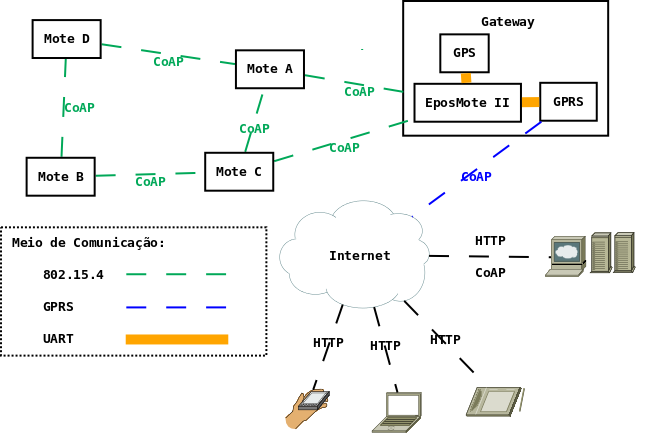
\includegraphics[width=0.8\textwidth]{figuras/arquitetura.png}
   \caption{Vis\~ao geral sobre comunica\c{c}\~ao do sistema.}
   \label{arquitetura}
\end{figure}

\subsection{Componentes}
A aplica\c{c}\~ao do gateway \'e composta por: Mecanismos de temporiza\c{c}\~ao, camada UDP/IP, parser de pacote CoAP, conjunto de comandos AT, Estruturas de filas, \textit{Hash} simples e \textit{Threads}.

A implementa\c{c}\~ao consiste num m\'odulo que trata requisi\c{c}\~oes, encapsula em pacotes e transmite por mecanimos de transmiss\~ao baseados em \cite{draft-ietf-core-coap-18}.

A biblioteca utilizada para montar o pacote CoAP foi a biblioteca CantCoap com algumas corre\c{c}\~oes e testes para facilitar a verifica\c{c}\~ao da execu\c{c}\~ao correta dos algoritmos internos durante o desenvolvimento da aplica\c{c}\~ao. As altera\c{c}\~oes resultaram em contribui\c{c}\~ao para o referido projeto, aceita pelo mantenedor.

Para o funcionamento desta biblioteca no EPOS e utilizar uma MTU limitada a 128 bytes foi utilizado um buffer com um valor m\'aximo para armazenamento dos dados do pacote no buffer. Foi necess\'ario alterar tipos das vari\'aveis para se adequarem ao EPOS.

No mecanismo de requisi\c{c}\~o e resposta, as requisi\c{c}\~oes pendentes foram armezenadas num \textit{Hash} com a chave sendo o token gerado pelo cliente. O protocolo CoAP foi modelado conforme \'e mostrado na figura \ref{uml} abaixo:
\begin{figure}[H]
   \centering
   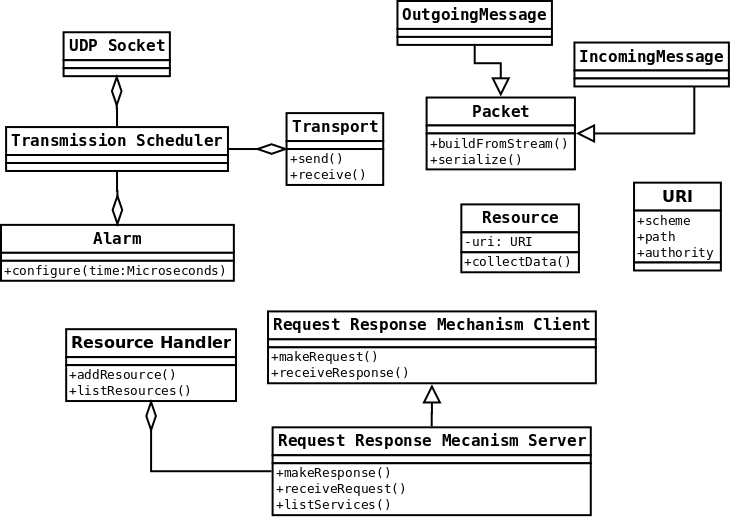
\includegraphics[width=0.8\textwidth]{figuras/uml.png}
   \caption{Diagrama UML das entidades de software implementadas.}
   \label{uml}
\end{figure}

A figura \ref{casodeuso} mostra o diagrama de caso de uso das principais fun\c{c}\~oes desenvolvidas.
\begin{figure}[H]
   \centering
   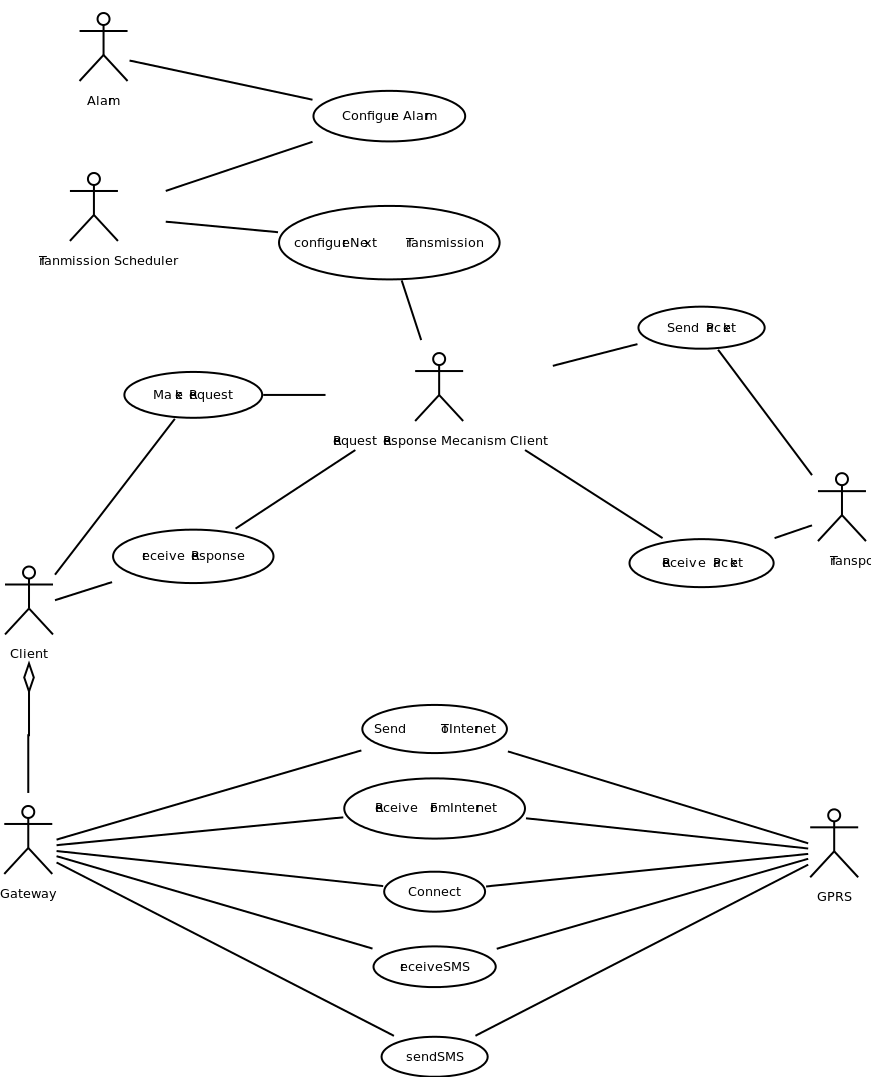
\includegraphics[width=0.7\textwidth]{figuras/casodeuso.png}
   \caption{Diagrama de casos de uso.}
   \label{casodeuso}
\end{figure}

A aplica\c{c}\~ao desenvolvida no EPOS utiliza buffer para o recebimento de dados da rede 802.15.4 que ser\'a enviado para rede via GPRS. Foram utilizadas duas threads, uma produtora que ficar\'a escutando o r\'adio 802.15.4 e outra consumidora que ser\'a respons\'avel em utlizar estes dados na rede de sensores e encaminh\'a-los pra Internet usando a extens\~ao GPRS do EPOSmote II. Para validar o comportamento foram utilizados testes da pr\'opria biblioteca CoAP portados para o EPOS.

No desenvolvimento do mecanismo de retransmiss\~ao de mensagens n\~ao-confirmadas foi utilizado uma lista ordenada e alarme configurado para o pr\'oximo reenvio. A figura \ref{diagramaSequenciaCoapClient} ilustra a intera\c{c}\~ao entre os m\'odulos de software, incluindo os tipos dos dados e a forma de execu\c{c}\~ao das fun\c{c}\~oes.

\begin{figure}[H]
   \centering
   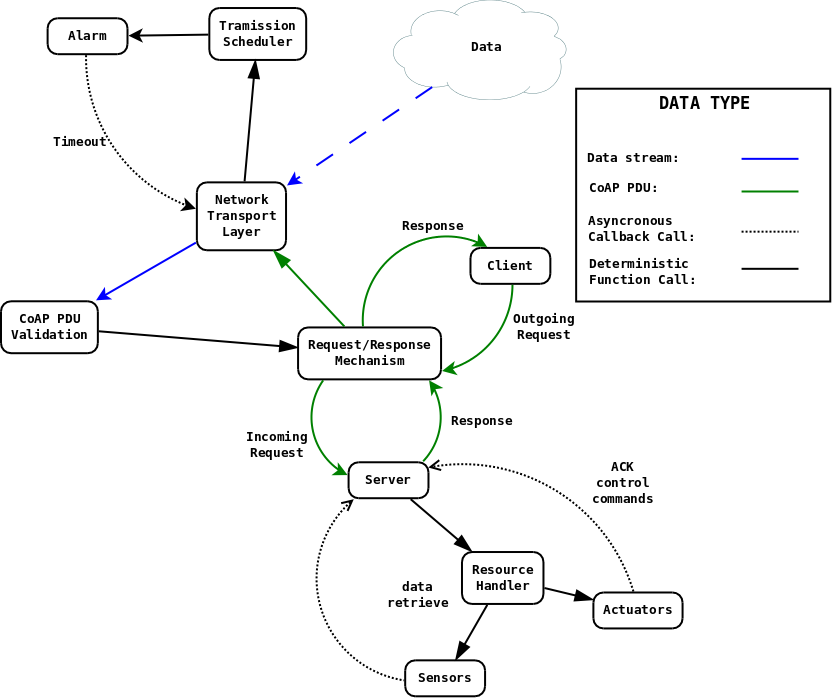
\includegraphics[width=1.0\textwidth]{figuras/coap.png}
   \caption{Abstra\c{c}\~ao dos m\'odulos de software da aplica\c{c}\~ao gateway.}
   \label{diagramaSequenciaCoapClient}
\end{figure}


\section{Implementa\c{c}\~ao}

A modelagem da solu\c{c}\~ao visa uma implementa\c{c}\~ao modular, para facilitar a verifica\c{c}\~ao do correto funcionamento e tamb\'em para ser de f\'acil adapta\c{c}\~a a diversas plataformas. O sistema proposto \'e composto pela aplica\c{c}\~ao gateway, por um servidor coap externo e um servidor http externo, este apenas para facilitar o acesso de dispositivos sem suporte ao protocolo CoAP.

O c\'odigo desenvolvido do servidor CoAP externo e o c\'odigo de sistema da plataforma alvo est\~ao dispon\'iveis em \cite{coapGatewayCode}.

Na inicializa\c{c}\~ao do m\'odulo 802.15.4, \'e feita a descoberta de servi\c{c}os, enviando um broadcast para os n\'os da rede de sensores sem fio. A figura abaixo \ref{onStartup}, demonstra o diagrama de sequ\^encia durante o processo de incializa\c{c}\~ao da aplica\c{c}\~ao gateway.  

\begin{figure}[H]
   \centering
   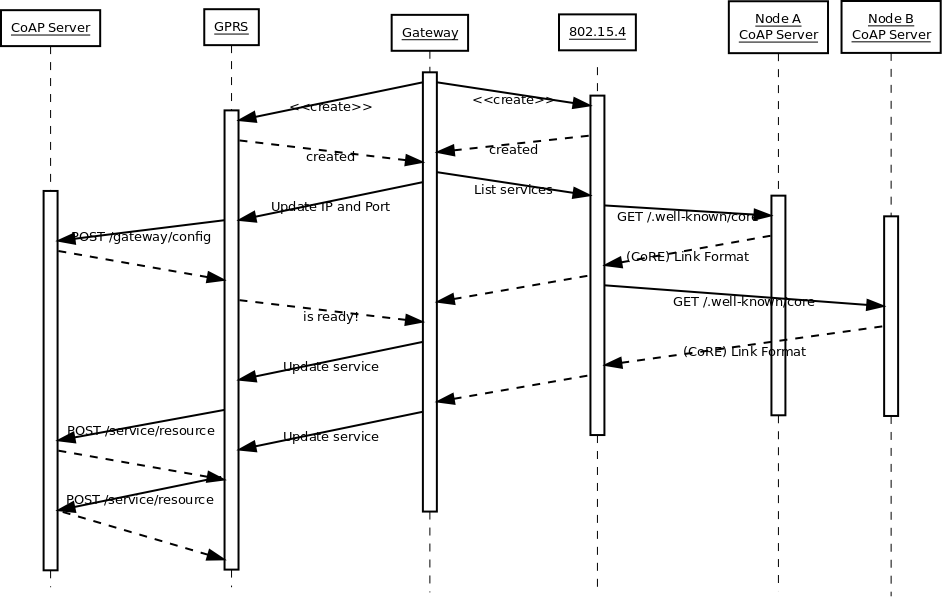
\includegraphics[width=1.0\textwidth]{figuras/umlOnStartup.png}
   \caption{Inicializa\c{c}\~ao do sistema.}
   \label{onStartup}
\end{figure}

No m\'odulo gateway, o sistema desenvolvido possui como entradas sequ\^encias de caracteres recebidos do transceiver 802.15.4 e m\'odulo GPRS, que s\~ao validados em pacotes CoAP. Ao estabelecer o t\'unnel e obter um endere\c{c}o IP e uma porta da rede m\'ovel \'e enviada uma requisi\c{c}\~ao CoAP para o recurso coap://hostname/gateway/config, contendo um JSON com o endere\c{c}o IP e a porta dispon\'iveis.

Ao receber uma mensagem pelo m\'odulo GPRS e validado o pacote CoAP \'e repassado para a rede de sensores conectada.  No caso de receber uma mensagem por 802.15.4, esta mensagem \'e validada e repassada para o hostname anteriormente definido no sistema.

Com isto o sistema est\'a apto para receber requisi\c{c}\~oes externas e enviar para a rede de sensores, quando a resposta retornar da RSSF, o pacote tamb\'em \'e validado e depois enviado para o endere\c{c}o previamente configurado.

O servidor CoAP utiliza a biblioteca Node-CoAP que recebe requisi\c{c}\~oes e repassa os pacotes para o endere\c{c}o da aplica\c{c}\~ao gateway, caso este esteja conectado na rede m\'ovel. Este servidor foi desenvolvido utilizando a linguagem JavaScript.

A aplica\c{c}\~ao gateway foi desenvolvida em C++, utilizando a biblioteca CantCoap pra montar os pacotes e alguns utilit\'arios do sistema operacional EPOS, como alarmes, listas ordenadas entre outros.

\section{Testes}
Durante o desenvolvimento foram realizados in\'umeros testes para verificar e validar o correto comportamento dos componentes de software e hardware.  A implementa\c{c}\~ao do protocolo CoAP foi testada da seguinte maneira:

\begin{description}
    \item[Testes unit\'arios:] Testes de constru\c{c}\~ao de pacotes v\'alidos e inv\'alidos utilizando como entrada sequ\^encia de caracteres e tratamento de respostas v\'alidas e inv\'alidas.
    \item[Testes de integra\c{c}\~ao:] Testes de interoperabilidade entre as implementa\c{c}\~oes, utilizando cen\'arios parecidos com o IOT Plugtest.
\end{description}

Os procedimentos para testar o m\'odulo GPRS foram: Enviar e recebimento de mensagens; criar socket UDP e TCP, enviar e receber mensagem via socket, fazer requisi\c{c}\~ao e receber respostas HTTP.
